\subsection{Opgaver}
\begin{enumerate}
	\item Løs differentialligningerne
	\begin{align*}
	y'=3,&&y'=\sin(x),&&y'=e^{-2x},
	\end{align*}
	alle med begyndelsesbetingelser $y(0)=2$.
	
	\item Bestem løsningen til differentialligningen
	\begin{align*}
	y'=-y
	\end{align*}
	som går gennem punktet $(1,\frac{1}{e^2})$. 
	
	\item Differentialligningen
	\begin{align*}
	y'=\frac{x+2y}{3},
	\end{align*}
	har en løsning som går gennem punktet $(1,3)$. Bestem en ligning for tangenten til løsningen i dette punkt.

	\item Løs følgende differentialligninger med begyndelsesbetingelser
\begin{enumerate}
	\item $y'=3x^3-1$, $y(0)=-1$.
	\item $y'-y=0$, $y(0)=\sqrt{2}$.
	\item $3y'+y=0$, $y'(0)=1$.
\end{enumerate}	
	
		\item Differentialligningen
	\begin{align*}
	y'=x-y^2,
	\end{align*}
	har en løsning som går gennem punktet $(3,5)$. Bestem en ligning for tangenten til løsningen i dette punkt.
	
		\item\label{it:diffeq21} For at få en forståelse for hvordan løsningerne til en differentialligning kan se ud kan man tegne såkaldte linjeelementer. Måden man gør det på er ved at udvælge punkter og så for hvert punkt tegne en linje med samme hældning som løsningen vil have i punktet. 
	
	I Figur~\ref{fig:diffeq21} ses en skitse af linjeelementer tilhørende differentialligningen
	\begin{align*}
	y'=x+y,
	\end{align*}
	samt grafen for løsningen med begyndelsesbetingelse $y(0)=1$. Skitser grafen for løsningen med begyndelsesbetingelser
	\begin{enumerate}
		\item $y(0)=0$.
		\item $y(0)=-1$.
		\item $y(0)=-2$.
	\end{enumerate}
	
	
	\begin{figure}
		\centering
		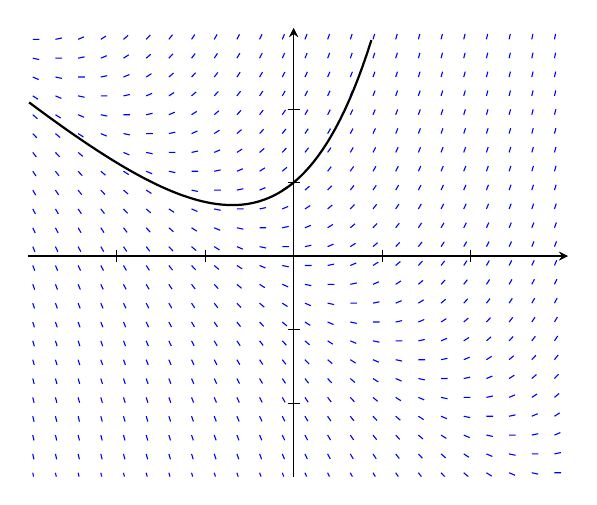
\begin{tikzpicture}[
		declare function={f(\x,\y) = \y+\x;} % Define which function we're using
		]
		\begin{axis}[
		axis x line=center,axis y line=center	,xmin=-3, xmax=3.1, % Axis limits
		ymin=-3, ymax=3.1,view={0}{90},xtick={-2,-1,0,1,2}, ytick={-2,-1,0,1,2},every x tick/.style={black},every y tick/.style={black},restrict y to domain=-3:3,restrict x to domain=-3:3]
		\def\length{sqrt(1+(f(x,y)^2)}
		\addplot3[blue, quiver={u={1/(\length)}, v={(f(x,y))/(\length)}, scale arrows=0.075},samples=40] {0};
		\addplot[thick,black,samples=200] {2*e^x-x-1};
		%		\addplot[thick,blue,samples=200] {e^x-x-1};
		%		\addplot[thick, red,samples=200] {-x-1};
		%		\addplot[thick,green,samples=200] {-e^x-x-1};
		%\addplot {x^2+0.15}; % You need to find the antiderivative yourself, unfortunately. Good exercise!
		\end{axis}
		\end{tikzpicture} 
		\caption{Opgave~\ref{it:diffeq21}}
		\label{fig:diffeq21}
	\end{figure}
	
		\item Differentialligningen
	\begin{align*}
	y'=\frac{x}{1+y^2},
	\end{align*}
	har en løsning som går gennem punktet $(4,1)$. Bestem en ligning for tangenten til løsningen i dette punkt.
	
	
	\item I Opgave~\ref{it:diffeq11} så vi at den fuldstændige løsning til differentialligningen
	\begin{align*}
	y'=ky
	\end{align*}
	er givet ved $y=ce^{kx}$ hvor $c\in \R$. Bestem løsninger som opfylder begyndelsesbetingelserne
	\begin{enumerate}
		\item $y(0)=a$.
		\item $y'(0)=b$.
	\end{enumerate}
	
	
	\item Differentialligningen
	\begin{align*}
	y'=3\sqrt{xy},
	\end{align*}
	har en løsning som går gennem punktet $(1,4)$. Bestem en ligning for tangenten til løsningen i dette punkt.
	

	
	
	
	\item Differentialligningen
	\begin{align*}
	y'=\frac{y-1}{x},
	\end{align*}
	har en løsning som går gennem punktet $(2,7)$. Bestem en ligning for tangenten til løsningen i dette punkt.
	
	\item \label{it:diffeq22}	 I Figur~\ref{fig:diffeq22} ses en skitse af linjeelementer tilhørende differentialligningen
	\begin{align*}
	\frac{y'}{y}=x^2-x,
	\end{align*}
	samt grafen for løsningen med begyndelsesbetingelse $y(0)=2$. Skitser grafen for løsningen med begyndelsesbetingelser
	\begin{enumerate}
		\item $y(0)=1$.
		\item $y(0)=-1$.
		\item $y(0)=-2$.
	\end{enumerate}
	
	
	\begin{figure}
		\centering
		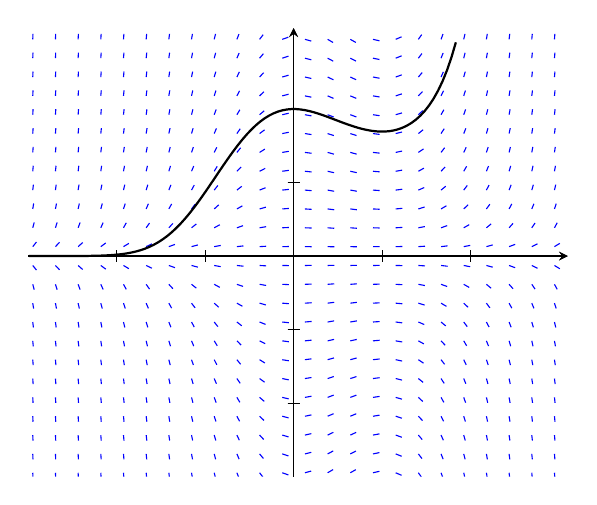
\begin{tikzpicture}[
		declare function={f(\x,\y) = \y*(\x*\x-\x);} % Define which function we're using
		]
		\begin{axis}[
		axis x line=center,axis y line=center	,xmin=-3, xmax=3.1, % Axis limits
		ymin=-3, ymax=3.1,view={0}{90},xtick={-2,-1,0,1,2}, ytick={-2,-1,0,1,2},xticklabels={$-2$,$-1$,$0$,$1$,$2$},restrict y to domain=-3:3,restrict x to domain=-3:3,every x tick/.style={black},every y tick/.style={black}]
		\def\length{sqrt(1+(f(x,y)^2)}
		\addplot3[blue, quiver={u={1/(\length)}, v={(f(x,y))/(\length)}, scale arrows=0.075},samples=40] {0};
		\addplot[thick,black,samples=200] {2*e^(x^2*(2*x-3)/6)};
%		\addplot[thick,blue,samples=200] {1*e^(x^2*(2*x-3)/6)};
%		\addplot[thick, red,samples=200] {0*e^(x^2*(2*x-3)/6)};
%		\addplot[thick,green,samples=200] {-1*e^(x^2*(2*x-3)/6)};
%		\addplot[thick,green,samples=200] {-2*e^(x^2*(2*x-3)/6)};
		\end{axis}
		\end{tikzpicture}
		\caption{Opgave~\ref{it:diffeq22}}
		\label{fig:diffeq22}
	\end{figure}
	
	
	
	\item Lad $f(x)$ være med en stamfunktion $F(x)$. Vis at funktionen 
	\begin{align*}
	g(x)=y_0+\int_{x_0}^x f(x)\dd x
	\end{align*}
	løser differentialligningen 
	\begin{align*}
	y'=f,
	\end{align*}
	med begyndelsesbetingelsen $y(x_0)=y_0$.
	
	
	
	
	
	
	
	
	
\end{enumerate}